\documentclass{ctexart}
\usepackage{amsmath,amssymb,amsthm,bm,ulem,graphicx}
\usepackage[margin=1 in]{geometry}
\title{数值分析作业2}
\author{数91\and 董浚哲\and 2019011985}
\begin{document}
\maketitle
\newcommand{\R}{\mathbf{R}}
\newcommand{\dd}{\,\mathrm{d}}
\newcommand{\st}{\text{ s.t. }}
\newcommand{\pp}[2]{\frac{\partial #1}{\partial #2}}
\newcommand{\nm}[1]{\left\|#1\right\|}

\paragraph{1.}
\subparagraph{(1)}
\begin{proof}
\begin{enumerate}
\item 由定义,显然$\mu(A)\geq 0$,等号成立当且仅当$A=0$
\item $\mu(\alpha A)=n\max\limits_{1\leq i,j\leq n}|\alpha a_{i,j}|\leq \alpha n\max\limits_{1\leq i,j\leq n}| a_{i,j}|$, $\mu(A)=n\max\limits_{1\leq i,j\leq n}|\frac{1}{\alpha}\alpha a_{i,j}|\leq \frac{1}{\alpha}\mu(A)$,故$\mu(\alpha A)=\alpha\mu(A)$
\item $\mu(A+B)=n\max\limits_{1\leq i,j\leq n}|a_{ij}+b_{ij}|\leq n\max\limits_{1\leq i,j\leq n}|a_{ij}|+|b_{ij}|\leq n\max\limits_{1\leq i,j\leq n}|a_{ij}|+n\max\limits_{1\leq i,j\leq n}|b_{ij}|=\mu(A)+\mu(B)$
\item $\mu(AB)=n\max\limits_{1\leq i,j\leq n}|\sum\limits_{k=1}^na_{ik}b_{kj}|\leq n \sum_{k=1}^n\max\limits_{1\leq i,j\leq n}|a_{i,j}|\max\limits_{1\leq i,j\leq n}|b_{i,j}|=n^2n\max\limits_{1\leq i,j\leq n}|a_{i,j}|\max\limits_{1\leq i,j\leq n}|b_{i,j}|=\mu(A)\mu(B)$
\end{enumerate}
故$\mu(A)$为矩阵范数。
\end{proof}

\subparagraph{(2)}
单位矩阵的相容范数总为$1$,但$\mu(I)=n$,故不是相容范数。

\paragraph{2.}
\subparagraph{(1)}
经计算,$A$的特征值为:$2,2-\sqrt{a^2+1},\sqrt{a^2 + 1}+2$。欲使$A$正定,需要所有特征值为正,故$a$的范围为$a\in (-\sqrt{3},\sqrt{3})$
\subparagraph{(2)}
\[L=\begin{bmatrix}
\sqrt{2}&0&0\\
\frac{\sqrt{2}}{2}&\frac{\sqrt{6}}{2}&0\\
0&\frac{\sqrt{6}}{3}&\frac{2\sqrt{3}}{3}
\end{bmatrix}\]

\paragraph{3.}
\begin{proof}
$\nm{L}^2_2=\rho(LL^T)=\rho(A)=\nm{A}_2$。

上面最后一个等式是因为:因$A$对称正定,故$\exists Q\in O_n(\mathbf{C})\st QAQ^T=D$,其中$D=\mathrm{diag}\{\lambda_1,\lambda_2,\cdots,\lambda_n\}$,其中$\lambda_1\geq \lambda_2\geq\cdots\geq\lambda_n\geq 0$。注意到正定矩阵不改变2-范数,故$\nm{A}_2=\nm{D}_2=\lambda_1=\rho(A)$。
\end{proof}

\paragraph{4.}
\begin{proof}
$\forall 1\leq j\leq n, \nm{A}_p=\max\limits_{\nm{x}_p=1}\nm{\sum_{k=1}^n a_kx_k}_p\geq \nm{Ae_j}_p=\nm{a_j}_p$.

$\forall 1\leq i\leq n, \nm{A^{-1}}=\max\limits_{Ax=b,\nm{b}_p=1}\nm{x}_p|$。注意到$b=\frac{a_i}{\nm{a_i}_p},x=\frac{e_i}{\nm{a_i}_p}$满足$Ax=b, \nm{b}_p=1$,故$\nm{A^{-1}}_p\geq\nm{\frac{e_i}{\nm{a_i}_p}}_p=\frac{1}{\nm{a_i}_p}$。

综上两不等式可得$\mathrm{cond}(A)_p=\nm{A}_p\nm{A^{-1}}_p\geq \frac{\nm{a_j}_p}{\nm{a_i}_p}\quad \forall 1,j=1,\cdots,n$,取$\max$即得。
\end{proof}

\paragraph{5.}
\subparagraph{(i)}
$c=\nm{b}_2=2$,$\omega=(Pb-b)=[1,-1,-1,-1]$,$P=\begin{bmatrix}3/4&1/4&  1/4&  1/4\\
1/4&  3/4& -1/4& -1/4\\
1/4& -1/4&  3/4& -1/4\\
1/4& -1/4& -1/4&  3/4\end{bmatrix}$
\subparagraph{(ii)}
$G_2=\begin{bmatrix}\frac{\sqrt{2}}{2}&\frac{\sqrt{2}}{2}\\-\frac{\sqrt{2}}{2}&\frac{\sqrt{2}}{2}\end{bmatrix}$,
$G_3=\begin{bmatrix}\frac{\sqrt{6}}{3}&\frac{\sqrt{3}}{3}\\-\frac{\sqrt{3}}{3}&\frac{\sqrt{6}}{3}\end{bmatrix}$,
$G_4=\begin{bmatrix}\frac{\sqrt{3}}{2}&\frac 1 2\\-\frac 1 2&\frac{\sqrt{3}}{2}\end{bmatrix}$,$P=G_4G_3G_2$

\paragraph{6.}
以$G_{k,l}$表示对第$k,l$行作Givens变换,使得第$k$行第一列的元素变为$0$。则$Q'=\mathrm{diag}\{I_{n-2},G_{n,1}\}\cdots\mathrm{diag}\{I_2,G_{n,1}\}\mathrm{diag}\{1,G_{n,1}\}G_{n,1}G_{2,n}\cdots G_{n-2,n}G_{n-1,n}$。即先利用最后一行从下到上消去第一列的元素而不引入下三角上的元素,再逐次利用第$1\sim n-1$行消去最后一行除对角元外的元素。

计算量:每次计算Givens变换的系数需10次计算,每次计算每涉及到非零的一列便需要6次计算。从下到上共$n-1$次变换,每次变换涉及$2,3,\cdots,n$个非零列。从上到下共$n-1$次变换,每次变换涉及$n,\cdots,2$个非零列,故总计$2(n-1)*10+6*(n-1)*(n+2)=6n^2+26n-32$次计算。


\paragraph{7.}
\subparagraph{(i)}
记$\hat{U}=
\begin{bmatrix}
\frac{1}{\sqrt{3}}&\frac{1}{\sqrt{2}}&\frac{1}{\sqrt{6}}\\
-\frac{1}{\sqrt{3}}&0&\frac{\sqrt{6}}{3}\\
\frac{1}{\sqrt{3}}&-\frac{1}{\sqrt{2}}&\frac{1}{\sqrt{6}}\end{bmatrix}$, $\hat{S}=\begin{bmatrix}-\sqrt{2}\alpha&0\\0&\sqrt{2}\\ 0& 0\end{bmatrix}$,则$A=\hat{U}\hat{S}V^T$。注意到$\hat{U},V$为正交矩阵不改变2-范数,故原问题等价于求解$\min\limits_x\nm{SV^Tx-U^Tb}$,其中$U^Tb=[0,2\sqrt{2},\sqrt{6}]^T$。记$b_1=[0,2\sqrt(2)]^T$,则$x=VS^{-1}b_1=[1,\sqrt{3}]'$

\subparagraph{(ii)}
既知$A$的SVD分解如上,则知其条件数在2-范数下为$\frac{\sigma_{max}}{\sigma_{min}}$,分子分母分别是最大、最小的非零奇异值。故
\begin{enumerate}
\item $\alpha\geq 1$时,$\kappa_2(A)=\alpha$
\item $\alpha<1$时,$\kappa_2(A)=\frac{1}{\alpha}$
\end{enumerate}

\subparagraph{(iii)}

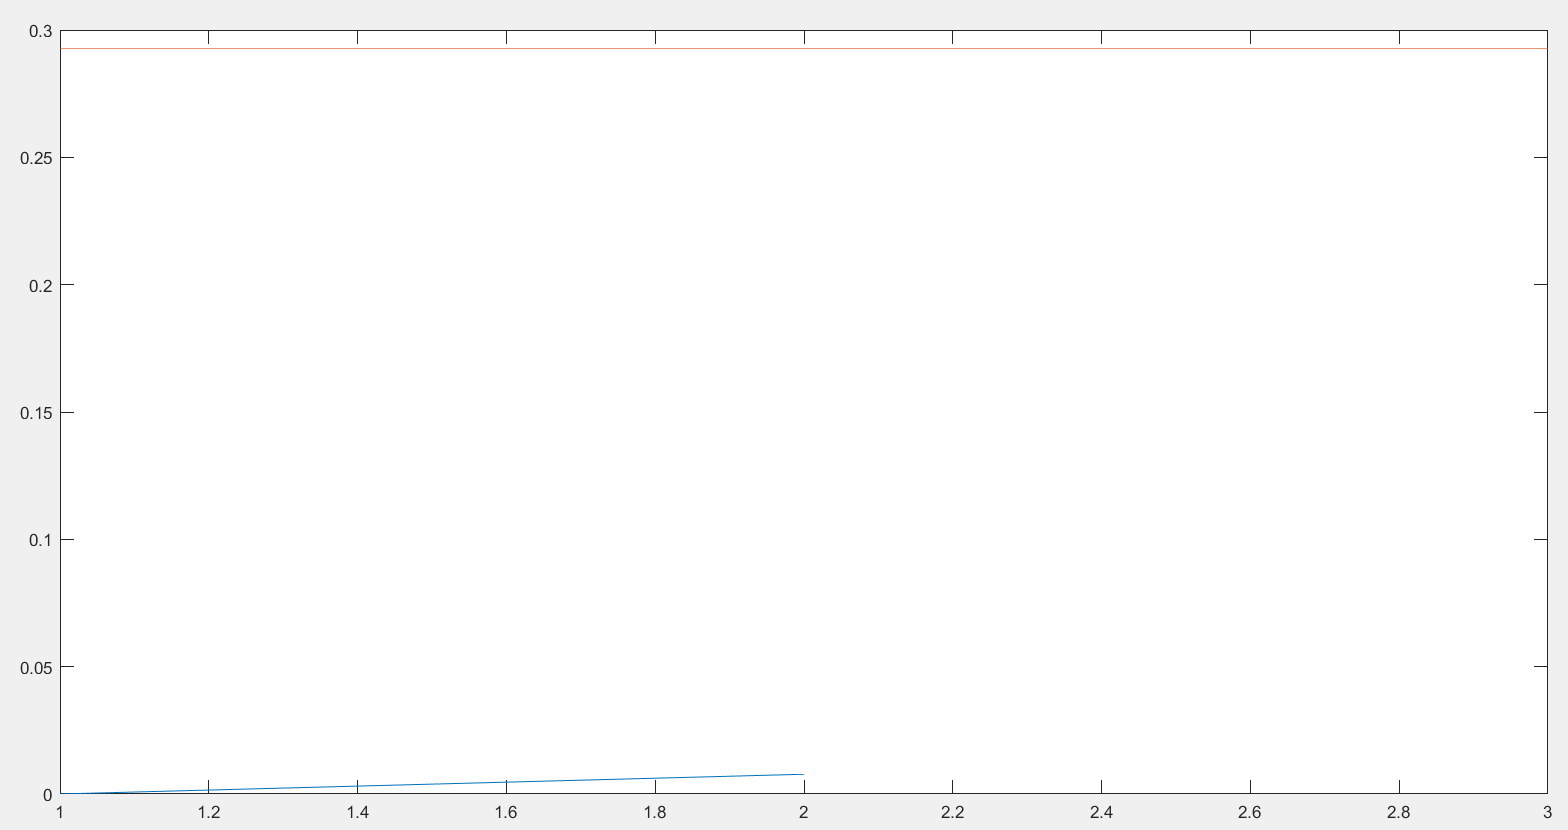
\includegraphics[scale=0.5]{2.7.1}

上图为$\nm{\cdot}_2$下的逐项相对误差,红线为QR分解而蓝线为Cholesky分解。

由于未经Pivoting,QR分解的稳定性反而不如使用稳定性较玄学的高斯消去法的Cholesky分解,至少有时是这样。








\end{document}